
\section{Context Description}
\section{Context Description}
This Chapter will identify global requirements for the system. These global requirements describe safety and functional behaviors which the system should fulfill at all times. To come to these requirements first a contextual description of the system is given taking simplifying assumptions into account.
\begin{figure}[!h]
	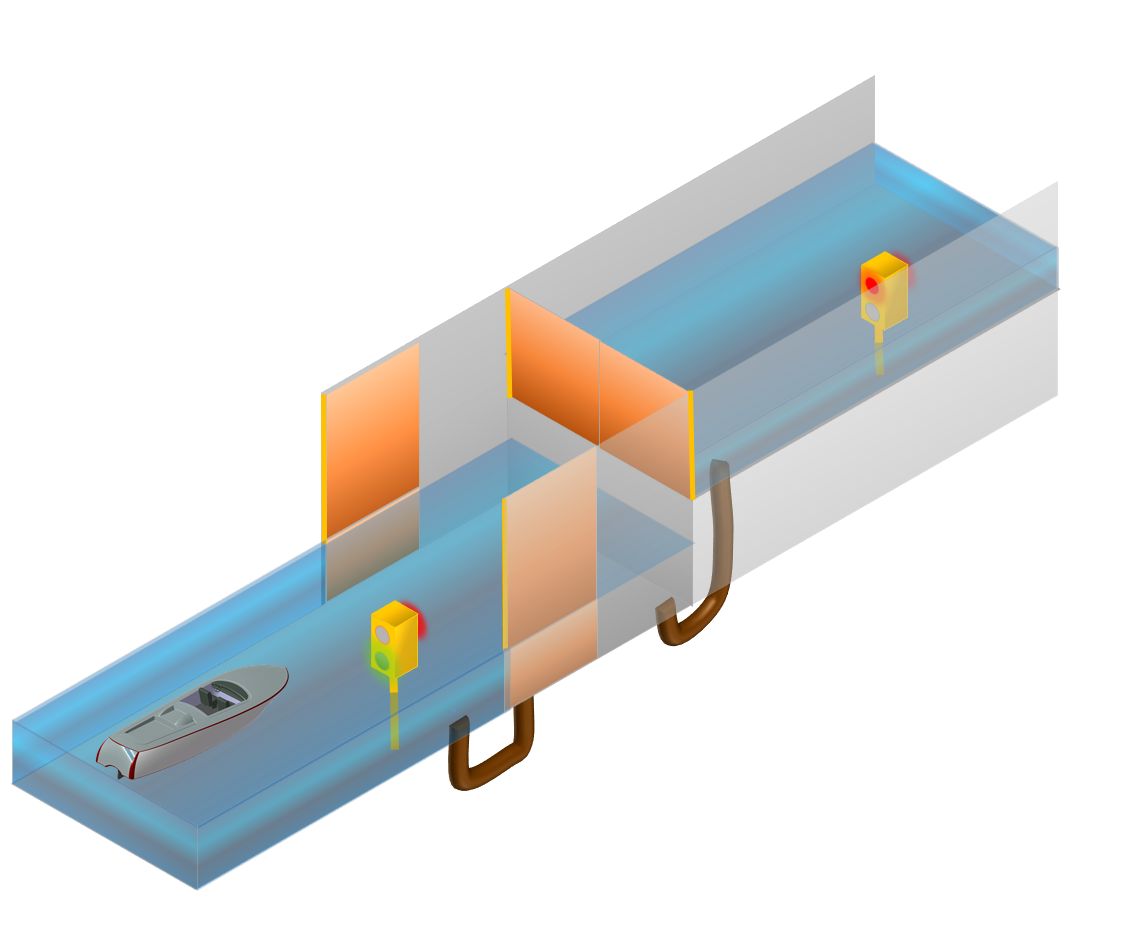
\includegraphics[width=\linewidth]{New}
	\caption{Ship lift.}
	\label{fig:boat1}
\end{figure}

\noindent
\\The system describes a ship lift that works through a sluice as depicted in \ref{fig:boat1}. A ship that wants to go or downstairs enters the corresponding basin through a gate that will be opened. This gate will then be shut. The water level is changed accordingly be opening of the two valves. Once the water level is equal to destination basin the corresponding gate can be opened again. The assumptions are made that the sluice lift only has two levels, with two corresponding gates, and two valves. Also the system should work completely autonomous. Furthermore there are two signaling systems, each facing both ways. Finally the assumptions are made that there is an unlimited supply of water coming from upstream and the Shiplift is big enough for all ships passing through. \\
\subsection{General Outline}
\begin{itemize}
	\item no operator - fully autonomous system
	\item only 2 two levels
	\item two gates
	\item two signaling systems, each facing both ways
	\item one valve per gate
	\item unlimited water supply on upper level
	\item Lift is assumed to be big enough for all ships passing through
\end{itemize}
\pagebreak


%
%\subsection{Output}
%\begin{enumerate}
%	\item Signal light: pass or hold
%	\item Gates: open or closed
%	\item Valves: open or closed
%\end{enumerate}
%
%\subsection{Input}
%\begin{enumerate}
%	\item Actuator states
%	\begin{itemize}
%		\item Signal light: pass or hold
%		\item Gates: open or closed
%		\item Valves: open or closed
%	\end{itemize}
%	\item Waterflow through valve pipes
%	\item Location of the ship in the system
%	\begin{itemize}
%		\item completely in the lift
%		\item at the signal lights
%	\end{itemize}
%\end{enumerate}
